% @author Yi Zhu, yi.zhu@berkeley.edu
% v1 October 01, 2019
% v2 May 27, 2020

\documentclass[11pt]{article}
\usepackage[utf8]{inputenc}
\usepackage[letterpaper, portrait, margin=1in]{geometry}
\usepackage{amsmath}
\usepackage{physics}
\usepackage{esint}
\usepackage{graphicx}
\usepackage{parskip}
\usepackage[dvipsnames]{xcolor}
\usepackage[colorlinks=true]{hyperref}
\definecolor{dmb}{HTML}{003366}
%\renewcommand{\section}[1]{\vspace{0.4cm}\large\textcolor{violet}{\underline{\textbf{#1}}}}

\begin{document}

\begin{center}
    \huge \textbf{An Introduction to \LaTeX}\\{\LARGE Undergraduate Laboratory at Berkeley, Physics \& Astronomy}
\end{center}

\section{What is LaTeX?}

LaTeX is a typesetting language that allows us to produce well formatted documents through plain text commands. These commands---stored in a TEX file---are then compiled into a PDF. \textit{This seems like a lot of work, why can't we use just use Microsoft Word?}

\textbf{Advantages of using LaTeX}
\begin{enumerate}
    \item Typesetting mathematical formulae is convenient and effective.
    \item Complex structures such as table of contents, bibliographies, etc., are easily generated.
    \item LaTeX encourages authors to write well-structured texts.
\end{enumerate}

\section{How to use \href{https://www.overleaf.com/read/bdvjgzpbvchk
}{this guide}}

For the sake of brevity, we will introduce a number of commands but do not show their effect. You should follow along on \hyperref[overleaf]{Overleaf}, typing each command you encounter. Do not memorize; rather, \textit{learn by doing.} 

\section{Syntax}

Commands begin with a backslash. Required arguments are placed in curly brackets that follow the command and optional arguments are placed in square brackets.

{\color{blue}
\begin{verbatim}
    \command[optional arg]{required arg}
\end{verbatim}}
{\color{blue}
\begin{verbatim}
    $ \sqrt{2}    $       % square root of two
    $ \sqrt[3]{2} $       % cube root of two
\end{verbatim}}
An environment is a section of code surrounded by the commands {\color{blue}\verb|\begin{enviornment name}|} and {\color{blue}\verb|\end{enviornment name}|}. Depending on the type of environment, we can specify special properties or formatting for text within the {\color{blue}\verb|\begin{}|} and {\color{blue}\verb|\end{}|} commands. For example, we can use the enumerate environment to typeset an ordered list. 

{\color{blue}
\begin{verbatim}
    \begin{enumerate}
        \item % first item
        \item % second item 
    \end{enumerate}
\end{verbatim}}

Finally, a percent sign denotes a comment. Any characters in the line after the percent sign will be ignored by the compiler.

{\color{blue}
\begin{verbatim}
    % This is a comment!
\end{verbatim}}

\section{Preamble}

The preamble precedes the body or content of a document. This is the place to define the document type, specify extra packages, and set various parameters. The preamble must at minimum contain:

{\color{blue}\begin{verbatim}
    \documentclass[12pt]{article}
    \usepackage[utf8]{inputenc} 
\end{verbatim}}

Here {\color{blue}\verb|article|} specifies the type of document, the optional parameter {\color{blue}\verb|12pt|} sets the font size, and the command {\color{blue}\verb|\usepackage[utf8]{inputenc}|} specifies the encoding of the document. Note, these parameters are fairly standard.

Page size, orientation, and margins can be specified with the {\color{blue}\verb|geometry|} package:

{\color{blue}
\begin{verbatim}
    \usepackage[letterpaper, portrait, margin=1in]{geometry}
\end{verbatim}}

where {\color{blue}\verb|letterpaper|} specifies page size, {\color{blue}\verb|portrait|} specifies the orientation, and {\color{blue}\verb|margin=1in|} specifies the width of the margins.

\section{Body}

The content of your document must lie within the body:

{\color{blue}
\begin{verbatim}
    \begin{document}
        % your content
    \end{document}
\end{verbatim}}

The body always follows the preamble.

\section{Text}

Text typed into your editor will be converted into paragraphs. A new paragraph can be created by leaving a blank line between paragraphs (or with the {\color{blue}\verb|\par|} command). Multiple blank lines are treated as a single blank line.

Paragraphs are fully justified (flush with both the left and right margins) by default. Environments with different justifications {\color{blue}(\verb|center|}, {\color{blue}\verb|flushleft|}, and {\color{blue}\verb|flushright|)} can be specified within an environment. For example:

{\color{blue}
\begin{verbatim}
    \begin{center} 
        %text 
    \end{center}
\end{verbatim}}

By default, LaTeX indents all paragraphs except the first paragraph of a section. Useful commands (note: {\color{blue}\verb|\setlength|} must be placed in the preamble):

{\color{blue}
\begin{verbatim}
    \indent                         % indent paragraph
    \noindent                       % no indent
    \setlength{\parindent}{0 ex}    % no indent globally
\end{verbatim}}
\newpage
Useful commands for spacing:

{\color{blue}
\begin{verbatim}
    \\                              % line break
    \newline                        % same function as \\
    \newpage                        % page break
    \clearpage                      % page break and clear floating elements
    \medskip                        % vertical skip (space between paragraphs)
    \vspace{length}                 % vertical space
    \hspace{length}                 % horizontal space
\end{verbatim}}  

Text can be stylized with the commands:

{\color{blue}
\begin{verbatim}
    \textbf{}                       % bold
    \textit{}                       % italicized
    \underline{}                    % underline
    \emph{}                         % emphasized (similar to italicized)
\end{verbatim}}

Local text sizes can be specified with the command (in order from largest to smallest):

{\color{blue}
\begin{verbatim}
    \Huge
    \huge
    \LARGE
    \large
    \normalsize (default)
    \small
    \footnotesize
    \scriptsize
\end{verbatim}}

\section{Mathematics}

Inline expressions are placed between two dollar signs.

{\color{blue}
\begin{verbatim}
    Isn't it funny that $ 2 \cdot 2 = 2+2 = 2^2 $?
\end{verbatim}}

Out of line expressions that are not integrated into text are specified by:

{\color{blue}
\begin{verbatim}
    \[ expression \]                % without numbering
    \( expression \)                % with numbering
\end{verbatim}}

Some common mathematical expressions:

{\color{blue}
\begin{verbatim}
    a_{b}                           % a subscript b
    a^{b}                           % a to the power of b
    \frac{a}{b}                     % a over b
    \cdot                           % center dot
    \times                          % times symbol
    \int_{a}^{b}{x\,dx}             % integral from a to b of x dx
    \left( content \right)          % left and right parenthesis
    \alpha \Alpha                   % lowercase and uppercase Greek
\end{verbatim}}

The {\color{blue}\verb|amsmath|} and {\color{blue}\verb|physics|} packages provides additional utility

\section{Document structure}

Content in an {\color{blue}\verb|article|} type document can be partitioned into sections and subsections using the commands {\color{blue}\verb|\section{}|} and {\color{blue}\verb|\subsection{}|}. LaTeX automatically numbers sections and this numbering can be omitted by placing an asterisk after the command: {\color{blue}\verb|\section*{}|}.

Creating bibliographies in LaTeX will be discussed in detail during the workshop hosted by the library.

\section{Figures}

The following is sample syntax for inserting a simple figure (note: you must import the {\color{blue}\verb|graphicx|} package in the preamble):

{\color{blue}
\begin{verbatim}
    \begin{figure}[ht]
        \centering
        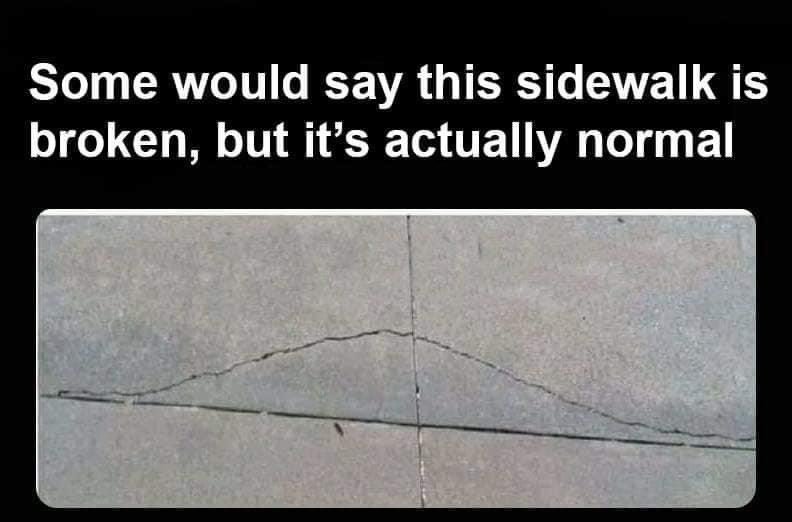
\includegraphics[width=0.25\textwidth, angle=45]{img}
        \caption{Image Caption}
    \end{figure}
\end{verbatim}}

The file path of the image is specified as a parameter of the {\color{blue}\verb|includegraphics|} command ({\color{blue}\verb|img|} in this case). If no file extension is provided, LaTeX will search all file types (this is recommended). 

Optional parameters can be provided to specify the scaling and rotation of the image. In our case, the image is scaled to quarter size and rotated counterclockwise by $45^\circ$). Furthermore, the centering command specifies that the image should be centered.

The optional arguments, {\color{blue}\verb|ht|}, for this figure environment specifies the relative position of the image. Some possible positioning parameters are:

{\color{blue}\begin{verbatim}
    h       % here
    t       % top of the page
    b       % bottom of the page
    H       % at this precise location (requires float package)
\end{verbatim}}

With parameter {\color{blue}\verb|ht|}, the typesetting engine will first try to place the figure at the current position. If the figure does not fit, the engine will try to shift text around so that the figure can be placed at the top of the page. 

\section{LaTeX compilers and IDEs}

In order to create and compile a TEX file on your computer, you will require (1) a TeX distribution and (2) a TeX editor\footnote{What is the difference between TeX vs. \LaTeX? TeX is the underlying typesetting language. LaTeX is a ``variant" of TeX with more user-friendly commands/features that are implemented via TeX macros.}. 

Common TeX distributions are MiKTeX for Windows, TeX Live for Linux, and MacTeX for Mac. Encapsulated within each TeX distribution is the typesetting engine\footnote{Commonly, pdfLaTeX or XeLaTex.} required to compile TEX files into PDFs.

While TEX files can be created in a plain-text editor, editors (IDEs) dedicated to LaTeX are generally more popular. Within these editors TEX files can be modified and compiled all at once. Popular editors include TeXstudio, Texmaker, GNU TeXmacs, etc.

\label{overleaf}LaTeX documents can also be created and compiled online via services like Overleaf. In ULAB, we will be using Overleaf because it does not require downloading software and allows for collaboration.

\section{Resources and debugging}

Google is a great resource for resolving errors and answering miscellaneous questions. Additionlly, Detexify, a handwritten LaTeX classification system is quite handy for the odd symbol: 

\url{http://detexify.kirelabs.org/classify.html}

\section{Bibliography}

A large portion of this material is drawn from, and inspired by, the Overleaf LaTeX Documentation (\url{https://www.overleaf.com/learn/latex/Main_Page}) and \textit{The Not So Short Introduction to \LaTeXe} by Tobias Oetiker, Hubert Partl, Irene Hyna and Elisabeth Schlegl.

\vspace{1 cm}
\centering
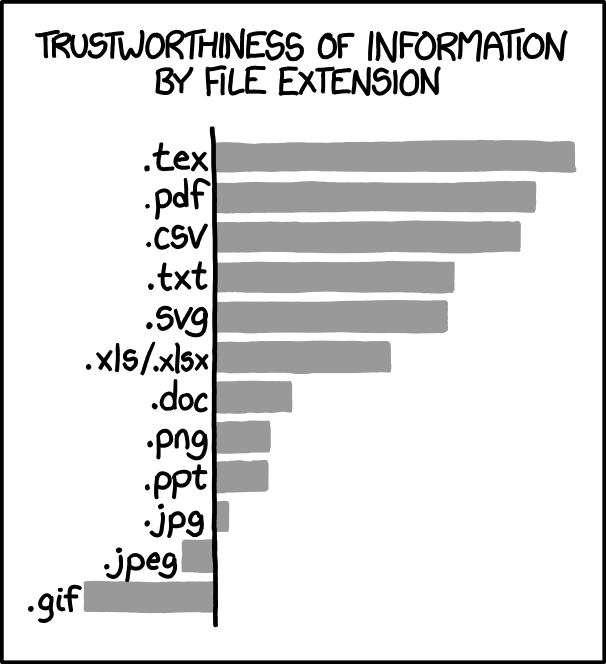
\includegraphics[width=0.45\textwidth]{xkcd}\\
https://xkcd.com/1301

\end{document}https://www.overleaf.com/read/pnfttnhcfhff